%%%%%%%%%%%%%%%%%%%%%%%%%%%%%%%%%%%%%%%%%
% Developer CV
% LaTeX Class
% Version 2.0 (12/10/23)
%
% This class originates from:
% http://www.LaTeXTemplates.com
%
% Authors:
% Omar Roldan
% Based on a template by  Jan Vorisek (jan@vorisek.me)
% Based on a template by Jan Küster (info@jankuester.com)
% Modified for LaTeX Templates by Vel (vel@LaTeXTemplates.com)
%
% License:
% The MIT License (see included LICENSE file)
%
%%%%%%%%%%%%%%%%%%%%%%%%%%%%%%%%%%%%%%%%%

%----------------------------------------------------------------------------------------
%	PACKAGES AND OTHER DOCUMENT CONFIGURATIONS
%----------------------------------------------------------------------------------------

\documentclass[9pt]{developercv} % Default font size, values from 8-12pt are recommended
\usepackage{multicol}
\setlength{\columnsep}{0mm}
%----------------------------------------------------------------------------------------
\usepackage{lipsum}  


\begin{document}

%----------------------------------------------------------------------------------------
%	TITLE AND CONTACT INFORMATION
%----------------------------------------------------------------------------------------

\begin{minipage}[t]{0.5\textwidth}
	\vspace{-\baselineskip} % Required for vertically aligning minipages

	{ \fontsize{16}{20} \textcolor{black}{\textbf{\MakeUppercase{Raihan Achmad D. F.}}}} % First name

	\vspace{6pt}

	{\Large Android $\sim$ Web Developer} % Career or current job title
\end{minipage}
\hfill
\begin{minipage}[t]{0.2\textwidth} % 20% of the page width for the first row of icons
	\vspace{-\baselineskip} % Required for vertically aligning minipages

	% The first parameter is the FontAwesome icon name, the second is the box size and the third is the text
	% \icon{Globe}{11}{\href{http://www.google.com}{portafolio.com}}\\ 
	% \icon{Phone}{11}{11 1111 1111}\\
	\icon{Envelope}{11}{\href{mailto:17radf@gmail.com}{17radf@gmail.com}}\\
	\icon{MapMarker}{11}{Indonesia}\\

\end{minipage}
\begin{minipage}[t]{0.27\textwidth} % 27% of the page width for the second row of icons
	\vspace{-\baselineskip} % Required for vertically aligning minipages

	% \icon{Envelope}{11}{\href{mailto:email@example.com}{email.email@example.com}}\\	
	\icon{Github}{11}{\href{https://github.com/raihanadf}{github.com/raihanadf}}\\
	\icon{LinkedinSquare}{11}{\href{https://www.linkedin.com/in/raihanadf}{/in/raihanadf}}\\

\end{minipage}

%----------------------------------------------------------------------------------------
%	INTRODUCTION, SKILLS AND TECHNOLOGIES
%----------------------------------------------------------------------------------------

\begin{minipage}[t]{0.20\textwidth}
	\vspace{-6pt}
	\vspace{5mm}
	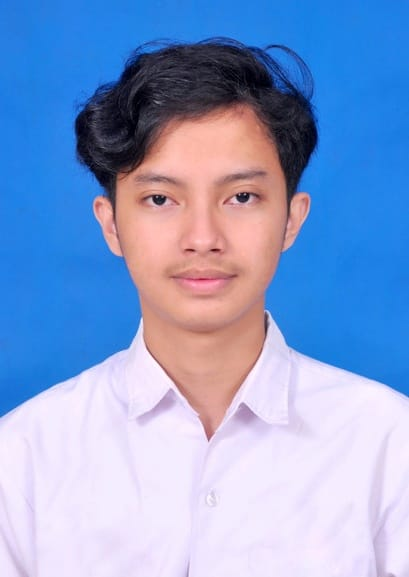
\includegraphics[width=4cm, height=6cm]{4x6.jpeg}
\end{minipage}
% \begin{minipage}[t]{0.30\textwidth}
% 	\cvsect{Summary}
% 	\vspace{-6pt}
%
% 	%Dummy text
% 	Raihan is an undergraduate student majoring in Informatics Engineering. He has experience in android and also web development with a passion for creating software solutions, is skilled in several programming languages, and is a self-taught Linux enthusiast.
%
% \end{minipage}
\hfill % Whitespace between
% \begin{minipage}[t]{0.70\textwidth}
%		\vspace{-6pt}
% \end
\begin{minipage}[t]{0.75\textwidth}

	\cvsect{Summary}
	\vspace{-6pt}

	%Dummy text
	Raihan is an undergraduate student majoring in Informatics Engineering. He has experience in android and also web development with a passion for creating software solutions, is skilled in several programming languages, and is a self-taught Linux enthusiast.

	\cvsect{Skills}
	\vspace{-6pt}

	\begin{minipage}[t]{0.2\textwidth}
		\textbf{Languages:}
	\end{minipage}
	\hfill
	\begin{minipage}[t]{0.73\textwidth}
		Java, JavaScript, Kotlin, Dart, PHP, SQL, NoSQL, Bash.
	\end{minipage}
	\vspace{4mm}

	\begin{minipage}[t]{0.2\textwidth}
		\textbf{Technologies:}
	\end{minipage}
	\hfill
	\begin{minipage}[t]{0.73\textwidth}
		Laravel, MariaDB, MongoDB, React.js, Node.js, Express.js, Android, Flutter, Tailwind, Material, LaTeX, Git.
	\end{minipage}
	\vspace{4mm}

	\begin{minipage}[t]{0.2\textwidth}
		\textbf{Soft Skills}
	\end{minipage}
	\hfill
	\begin{minipage}[t]{0.73\textwidth}
		Teamwork, Problem Solving, Time Management, Communication.
	\end{minipage}
	\vspace{4mm}

\end{minipage}

%----------------------------------------------------------------------------------------
%	EXPERIENCE
%----------------------------------------------------------------------------------------
\cvsect{Experience}
\begin{entrylist}
	\entry
	{02/2023 -- Present}
	{Freelance Laravel Developer}
	{Yayasan Pustaka Obor Indonesia}
	{
	Doing freelance maintaining a huge repository of book library management web app.
	\\ \texttt{Laravel} \slashsep \texttt{MariaDB} \slashsep \texttt{Filament}}
	\entry
	{08/2024 -- Present}
	{Full Stack Developer Intern}
	{PT Global Data Inspirasi (DataIns)}
	{
	Assisted by helping scraping some data, which will be used in matching fund program.
	\\ \texttt{NextJS} \slashsep \texttt{PostgreSQL}}
	\entry
	{08/2024 -- 08/2024}
	{Data Engineer Intern}
	{Badan Riset dan Inovasi Nasional RI (BRIN RI)}
	{
	Assisted by helping scraping some data, which will be used in matching fund program.
	\\ \texttt{Selenium}}
	\entry
	{02/2024 -- 07/2024}
	{Mobile Development Cohort}
	{Bangkit Academy led by Google, Tokopedia, Gojek, \& Traveloka}
	{Graduated with distinction (Top 100 Graduate).
	\\ \texttt{Android Views} \slashsep \texttt{Kotlin} \slashsep \texttt{SQLite} \slashsep \texttt{Koin}}
	\entry
	{06/2023 -- 12/2023}
	{Research Staff Intern}
	{PT. Bensae Kreasi Indonesia}
	{Involved in research of a VR-based simulator for post-stroke physiotherapy, focusing on the ergonomics of the interface and user experience. The research process follows a five-plane model and human-centered design methodology. Conducted Usability testing to evaluate the interface design and user experience.}
	\entry
	{01/2020 -- 03/2020}
	% \\\footnotesize{scholarship holder}
	{Digital Marketing Intern}
	{Primaland}
	{Learnt how to do "marketing" on Facebook and other marketplace and assisted Content Writer on publishing company products.}
	\entry
	{10/2019 -- 12/2019}
	% \\\footnotesize{scholarship holder}
	{Software Engineer Intern}
	{Primaland}
	{{Developed a real estate front-end website, and admin panel for the startup company. Collaboratively built an employee scoring system application with intern team.}
	\vspace{-7 pt}
	\\ \\
	{* was being an intern when I was on vocational high school.}
	\\
	\texttt{Framework7} \slashsep \texttt{PHP} \slashsep \texttt{SQL} \slashsep \texttt{Excel}}
\end{entrylist}

%----------------------------------------------------------------------------------------
%	VOLUNTEER
%----------------------------------------------------------------------------------------
\vspace{-10 pt}
\cvsect{Volunteer}
\begin{entrylist}
	\entry
	{08/2023 -- 08/2023}
	{Back End Developer}
	{KOICA}
	{Participating in "World Friends Korea" program between State Polytechnic of Jember and Kyungpook National University on the project named "The Smart Trash Bin". Built a web server that integrates the front-end and an Arduino for the team project.
	\vspace{-7 pt}
	\\ \\
	{* achieved 2nd place for the project.}
	}
\end{entrylist}


%----------------------------------------------------------------------------------------
%	EDUCATION
%----------------------------------------------------------------------------------------
\vspace{-10 pt}
\cvsect{Education}
\begin{entrylist}
	\entry
	{08/2021 -- 06/2025 \\\footnotesize{expected graduation}}
	{Informatics Engineering}
	{State Polytechnic of Jember}
	{Completed courses in data structures, algorithms, software engineering, web development, and system integration. Gained practical experience through internships and class projects, developing applications and systems for various industries.}
	\entry
	{07/2018 -- 06/2021}
	{Software Engineering}
	{Vocational High School State 1 of Bondowoso}
	{\vspace{-10pt}
		Ranked 3rd in 10th class. 2nd in 11th class. 1st in 12th class. And lastly,  6th in parallel class on graduation.
	}
\end{entrylist}

%----------------------------------------------------------------------------------------
%	Licenses & Certificate
%----------------------------------------------------------------------------------------
\vspace{-1 pt}
\cvsect{Licenses \& certifications}
\begin{entrylist}
	\entry
	{07/2024
		\\\footnotesize{BA24/DIST/XXIV-07\\/A129D4KY4396}}
	{Certificate of Completion}
	{Bangkit Academy led by Google, Tokopedia, Gojek, \& Traveloka}
	{Completed Bangkit, specializing in Mobile Development, with Distinction.}
	\entry
	{07/2024
		\\\footnotesize{TBI-DAGO/CORP/10439}}
	{English for Business Communication}
	{Dicoding Indonesia}
	{Completed a short course of 4.5 hours and achieved an overall score of 84\%}
	\entry
	{04/2024 -- 04/2027
		\\\footnotesize{07Z604KK2ZQR}}
	{Belajar Pengembangan Aplikasi Android Intermediate}
	{Dicoding Indonesia}
	{Covered advanced Android development: UI, animations, localization, services, media, geolocation, testing, databases, and Firebase. Completed with a story app project featuring photo-sharing and paging.}
	\entry
	{04/2024 -- 04/2027
		\\\footnotesize{RVZKR1DM4PD5}}
	{Belajar Penerapan Machine Learning untuk Android}
	{Dicoding Indonesia}
	{This course covered integrating machine learning in Android apps using MLKit, TensorFlow Lite, MediaPipe, and Firebase ML. It included a final project classifying images from the gallery on-device.}
	\entry
	{03/2024 -- 03/2027
		\\\footnotesize{KEXL85M8WZG2}}
	{Belajar Fundamental Aplikasi Android}
	{Dicoding Indonesia}
	{Completed a final project submission after studying the principles of Android app development, fragments, navigation components, background threading, networking, architecture components, testing, local data persistence, and background task scheduling.}
	\entry
	{03/2024 -- 03/2027
		\\\footnotesize{98XW2779JPM3}}
	{Belajar Membuat Aplikasi Android untuk Pemula}
	{Dicoding Indonesia}
	{Covered setting up Android Studio, creating activities with lifecycle management, using intents for debugging and activity transitions, designing layouts with a variety of view elements, implementing styles and themes, and integrating RecyclerView for list display.}
	\entry
	{03/2024 -- 03/2027
		\\\footnotesize{L4PQQDEJOPO1}}
	{Belajar Prinsip Pemrograman SOLID}
	{Dicoding Indonesia}
	{Understood five concept of SOLID and ready to implement it for developing apps.}
	\entry
	{03/2024 -- 03/2027
		\\\footnotesize{GRX5Q15VVZ0M}}
	{Memulai Pemrograman dengan Python}
	{Dicoding Indonesia}
	{Learned the fundamentals of Python and examined its control flow, data interaction, arrays, matrices, subprograms, optional OOP, style guide, unit testing, and popular libraries.}
	\entry
	{02/2024 -- 02/2027
		\\\footnotesize{2VX3OE4WVZYQ}}
	{Memulai Pemrograman dengan Kotlin}
	{Dicoding Indonesia}
	{44 hours were spent on the basics, control flow, object-oriented and functional programming, generics, special classes and collections, introduction to coroutines, and an examination of the background and importance of Kotlin.}
	\entry
	{02/2024 -- 02/2027
		\\\footnotesize{07Z6W7QNJZQR}}
	{Pengenalan ke Logika Pemrograman (Programming Logic 101)}
	{Dicoding Indonesia}
	{Studied computational thinking concepts, investigated logic and algorithms, examined logic gates, and implemented programming logic in practical situations.}
	\entry
	{11/2022 -- 11/2025
		\\\footnotesize{631202512300022...}}
	{Junior Mobile Programmer}
	{Badan Nasional Sertifikasi Profesi}
	{Learnt how layout, design \& theming, interactivity, assets \& media, navigating \& routing works on flutter. And a little bit of data \& backend too including state management (BLoC and Getx).}
	\entry
	{10/2022 -- 10/2025
		\\\footnotesize{EYX4911R5PDL}}
	{Belajar Membuat Front-End Web untuk Pemula}
	{Dicoding Indonesia}
	{Learnt how to build interactive front-end application that has storage feature using web storage as well.}
\end{entrylist}

%----------------------------------------------------------------------------------------
%	Projects
%----------------------------------------------------------------------------------------
\vspace{-10 pt}
\cvsect{Projects}
\begin{entrylist}
	\entry
	{Freelance Project}
	{ARECO}
	{Private Repo}
	{
		\vspace{-10 pt}
		\begin{itemize}[noitemsep,topsep=0pt,parsep=0pt,partopsep=0pt, leftmargin=-1pt]
			\item {A "Zoo" application that integrates with Unity and has quiz feature.}
		\end{itemize}
		\texttt{Flutter} \slashsep \texttt{BLoC}
	}
	\entry
	{Freelance Project}
	{Air Temperature}
	{https://github.com/raihanadf/air-temperature-app}
	{
		\vspace{-10 pt}
		\begin{itemize}[noitemsep,topsep=0pt,parsep=0pt,partopsep=0pt, leftmargin=-1pt]
			\item {Simple air monitoring app which integrated with IoT.}
		\end{itemize}
		\texttt{Flutter} \slashsep \texttt{Firebase} \slashsep \texttt{BLoC}
	}
	\entry
	{Freelance Project}
	{Pink Book}
	{https://github.com/raihanadf/pink-book-app}
	{
		\vspace{-10 pt}
		\begin{itemize}[noitemsep,topsep=0pt,parsep=0pt,partopsep=0pt, leftmargin=-1pt]
			\item {An app for tracking pregnancy health.}
		\end{itemize}
		\texttt{Flutter} \slashsep \texttt{Firebase} \slashsep \texttt{BLoC}
	}
	\entry
	{Contract Project}
	{Book Publishing Company Management System}
	{Private Repo}
	{
		\vspace{-10 pt}
		\begin{itemize}[noitemsep,topsep=0pt,parsep=0pt,partopsep=0pt, leftmargin=-1pt]
			\item {Collaboratively designed the system database and system architecture.}
			\item {Built and maintain payment and journaling system.}
		\end{itemize}
		\texttt{PHP} \slashsep \texttt{Laravel} \slashsep \texttt{Filament} \slashsep \texttt{Tailwind} \slashsep \texttt{SQL}
	}
	\entry
	{Semester Project}
	{Employee Attendance System}
	{github.com/raihanadf/java-presensi-non-pns}
	{\vspace{-10 pt}
		\begin{itemize}[noitemsep,topsep=0pt,parsep=0pt,partopsep=0pt, leftmargin=-1pt]

			\item {Built automatic attendance system for civil servant and "P3K" staff.}
			\item {Integrates the system with attending dates to each class and RFID for scanning.}
			\item {Designed the system database and collaborate with team on how to work with the system architecture and flows.}
		\end{itemize}
		\texttt{Java} \slashsep \texttt{NetBeans} \slashsep \texttt{SQL}}
	\entry
	{Semester Project}
	{Suki Mobile}
	{github.com/Ongghuen/suki-mobile}
	{\vspace{-10 pt}
		\begin{itemize}[noitemsep,topsep=0pt,parsep=0pt,partopsep=0pt, leftmargin=-1pt]
			\item Designed the User Interface and User Experience.
			\item Built a mobile app for suki furniture e-commerce. This includes payment, multiple transactions, items features such as searching, filtering, etc. Implementing state management with BLoC.
		\end{itemize}
		\texttt{Flutter} \slashsep \texttt{BLoC}}
	\entry
	{Semester Project}
	{Diskoperindag Mobile}
	{github.com/Ongghuen/diskoperindag-mobile}
	{\vspace{-10 pt}
		\begin{itemize}[noitemsep,topsep=0pt,parsep=0pt,partopsep=0pt, leftmargin=-1pt]
			\item Designed the User Interface and User Experience.
			\item Developed news feed system, notification, and training-tracking system. Implementing the application with recommended android architecture tools and pattern, this includes using navigation compose, fragments, viewmodel, binding, etc.
		\end{itemize}
		\texttt{Android} \slashsep \texttt{Material} \slashsep \texttt{Firebase}
	}
\end{entrylist}

%----------------------------------------------------------------------------------------
%	LANGUAGES
%----------------------------------------------------------------------------------------
\vspace{-10 pt}
\cvsect{Languages}
\vspace{-6pt}

\hspace{26mm} \textbf{English} - Professional working proficiency, \textbf{ Indonesian} - Native or bilingual proficiency
%----------------------------------------------------------------------------------------

\end{document}
